\documentclass[11pt]{article}
\usepackage[review]{acl}

\usepackage{amsmath}
\usepackage{amssymb}
\usepackage{booktabs}
\usepackage{multirow}
\usepackage{graphicx}
\usepackage{adjustbox}
\usepackage{subcaption}
\usepackage{enumitem}
\usepackage{placeins}
\usepackage{xeCJK}
\setCJKmainfont{Noto Serif CJK SC}
\setCJKsansfont{Noto Sans CJK SC}
\setCJKmonofont{Noto Sans Mono CJK SC}

\newcommand{\ours}{\textsc{ours}}

\title{When Meaning Dissolves: What Audio-Text Alignment Models Actually Encode}

\author{Anonymous}

\begin{document}

\maketitle

\begin{abstract}
Audio-text alignment models map text and audio into shared embedding spaces, but whether semantic content in text contributes to this alignment remains unclear. We investigate this using \emph{hachimi lyrics} (Chinese internet re-recordings that replace meaningful lyrics with nonsense syllables while preserving melody, instrumentation, and vocal timbre). Across 166 paired songs and three CLAP variants, we find that CLAP models show \emph{model-dependent} sensitivity to lyric surface form; preserving semantics or phonology alone is insufficient to predict alignment behavior. Specifically, meaning-preserving paraphrases of original lyrics produce alignment indistinguishable from originals in both LAION CLAP variants ($d{=}{-}0.02$ and $d{=}0.14$, both n.s.), while nonsense hachimi lyrics produce moderately higher alignment ($d{=}{-}0.24$ to $-0.37$, all $p{<}0.01$). Microsoft CLAP, by contrast, does distinguish paraphrases from originals ($d{=}0.45$), showing that paraphrase sensitivity is model-dependent rather than universal. All three models agree that paraphrases have lower alignment than hachimi text (LAION $d{=}{-}0.25$; LAION-Fused $d{=}{-}0.50$; msCLAP $d{=}{-}0.63$), while instrumental accompaniment attenuates this pattern in LAION CLAP ($d{=}{-}0.24$ full-mix vs.\ $d{=}{-}0.47$ vocal-only). Acoustic feature analysis identifies MFCC coefficients as the strongest alignment predictors (three survive Bonferroni correction, largest $|r|{=}0.36$), ZCA whitening eliminates all alignment (max${=}0.008$), and spectral perturbation analysis is consistent with spectral content influencing CLAP alignment. These results suggest that CLAP variants show nontrivial sensitivity to lyric surface form under Chinese perturbations; this sensitivity is not reducible to meaning-preserving paraphrase effects or pure phonology preservation.
\end{abstract}

% ============================================================
\section{Introduction}\label{sec:intro}
% ============================================================

Multimodal alignment models that map text and audio into shared embedding spaces are foundational to music information retrieval~\citep{wu2023clap}, video understanding~\citep{radford2021clip}, and cross-modal retrieval~\citep{yuan2023music}. These models are trained to align semantically meaningful text with corresponding audio, yet whether \emph{text semantics} actually contribute to this alignment has received limited direct testing. Research on pseudoword embeddings shows that language models encode structure even for non-lexical items~\citep{formanier2024meaning}, sound-symbolism studies reveal that CLIP-like models capture phonetic properties of nonsense syllables~\citep{masson2023kiki}, and cognitive science shows that phonological rather than semantic features drive the speech-to-song illusion~\citep{tierney2012phonological}. Despite this evidence, no prior work has used naturally occurring non-semantic text to directly test whether semantic content contributes to cross-modal alignment beyond what shared acoustic properties can explain.

We test this using \emph{hachimi lyrics}~(\textrm{哈基米歌词}), a Chinese internet culture phenomenon where popular songs are re-recorded with nonsense syllables such as ``ha-ji-mi'' (\textrm{哈基米}) and ``man-bo'' (\textrm{曼波}). These syllables have Chinese phonological structure but carry no stable meaning. The re-recordings preserve melody, instrumentation, and vocal timbre, giving a natural experiment where acoustic properties are held constant while semantic content is removed. Each hachimi song has an original version with meaningful lyrics, providing paired data for controlled comparison. Figure~\ref{fig:hachimi} illustrates this cultural phenomenon.

\begin{figure}[!t]
    \centering
    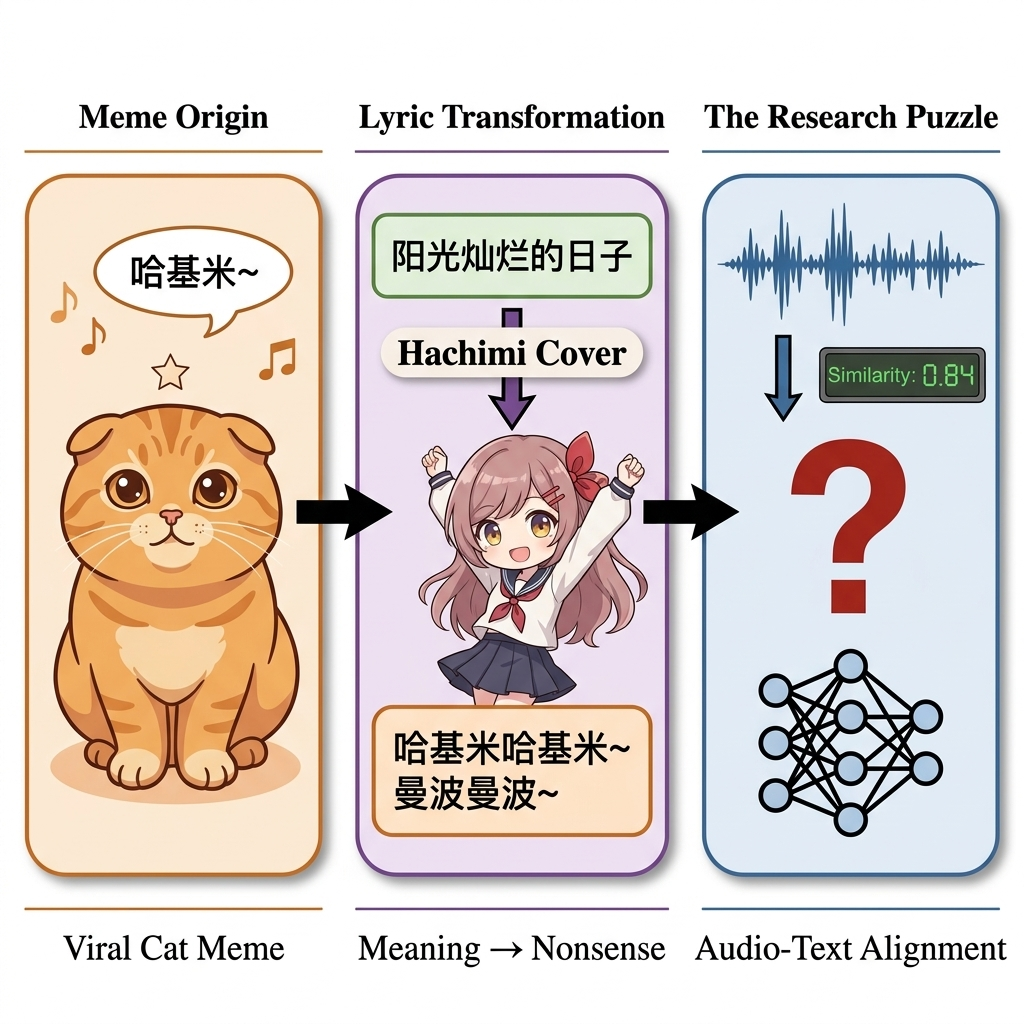
\includegraphics[width=\linewidth]{figures/fig_hachimi_intro.png}
    \caption{The \emph{hachimi} cultural phenomenon. \textbf{Left}: The meme originated from a viral cat video where ``ha-ji-mi'' (\textrm{哈基米}) was sung to a cute cat. \textbf{Center}: Internet users replace meaningful song lyrics with nonsense syllables (e.g., ``ha-ji-mi'', ``man-bo'') while preserving the original melody and instrumentation. \textbf{Right}: Despite the text becoming meaningless, audio-text alignment models still produce high similarity scores, raising the central research question of this paper.}
    \label{fig:hachimi}
\end{figure}

To test whether semantics contribute to alignment, we introduce a meaning-preserving paraphrase condition: an LLM rewrites original lyrics using different words while preserving identical meaning. If semantics drive alignment, paraphrases should match originals (same meaning, similar alignment) and differ from nonsense (different meaning, different alignment). If surface form drives alignment, paraphrases should differ from originals (different words) but match nonsense (both Chinese text). If neither matters, all three conditions should produce indistinguishable alignment.

Using 166 paired songs and a ten-condition degeneration spectrum, we measure alignment with three CLAP variants: LAION CLAP~\citep{wu2023clap} (512-dim, English-dominant training), its fused variant with cross-modal fusion layers, and Microsoft CLAP~\citep{elizalde2024msclap} (1024-dim, multilingual training). We extract 57-dimensional acoustic feature vectors to identify what influences alignment when semantics do not. Our contributions are:
(1)~\textbf{the first curated hachimi alignment dataset}, comprising 166 paired original--hachimi Chinese songs with ten systematically controlled text conditions and temporally matched audio segments --- to our knowledge, the first dataset to leverage naturally occurring nonsense lyrics for probing audio-text alignment;
(2)~evidence that CLAP variants show \emph{model-dependent} sensitivity to lyric surface form: both LAION CLAP variants treat meaning-preserving paraphrases identically to originals (standard: $d{=}{-}0.02$, $p{=}0.82$; fused: $d{=}0.14$, $p{=}0.08$), while Microsoft CLAP does distinguish them ($d{=}0.45$), showing that paraphrase sensitivity is not universal across CLAP variants;
(3)~evidence that all three models agree nonsense hachimi lyrics produce moderately higher alignment than originals ($d{=}{-}0.24$ to $-0.37$), and that instrumental accompaniment attenuates this pattern ($d{=}{-}0.24$ full-mix vs.\ $d{=}{-}0.47$ vocal-only in LAION CLAP);
(4)~identification of timbre (MFCC coefficients) as the strongest acoustic alignment predictor ($|r|{=}0.26$--$0.36$), with ZCA whitening eliminating all alignment (max${=}0.008$) and spectral perturbation analysis showing results consistent with spectral content influencing CLAP alignment.

\begin{figure*}[!t]
    \centering
    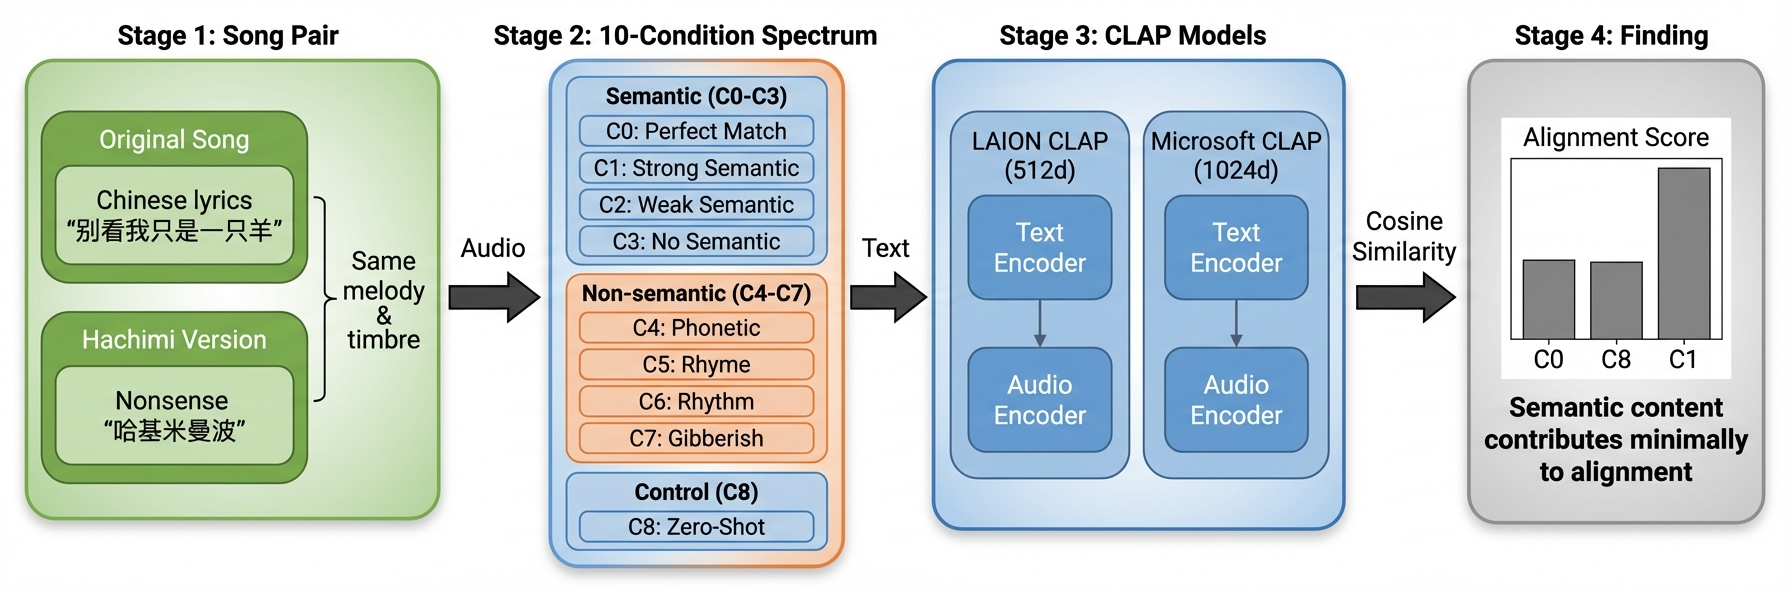
\includegraphics[width=\textwidth]{figures/fig_overview.png}
    \caption{\textbf{Overview of the hachimi probing approach.} Each original song (meaningful lyrics) is paired with a hachimi version (nonsense syllables ``ha-ji-mi'') that preserves melody, instrumentation, and vocal timbre. Ten text conditions (C0--C8) systematically vary semantic and structural integrity. Alignment is measured as cosine similarity between CLAP text and audio embeddings. The key finding: CLAP variants show model-dependent sensitivity to lyric surface form; preserving meaning or phonology alone is insufficient to predict alignment behavior.}
    \label{fig:overview}
\end{figure*}

% ============================================================
\section{Related Work}\label{sec:related}
% ============================================================

\subsection{Probing Multimodal Alignment}

Probing what contrastive vision-language models learn has become an active area. \citet{koishigarina2025clip} show that CLIP treats cross-modal matching as bag-of-words alignment, while \citet{bhalla2024splice} decompose CLIP's latent space into sparse linear concept combinations. \citet{zhang2024adversarial} demonstrate that multi-modal embeddings can be trivially perturbed to align any input with arbitrary text. In audio-text alignment, \citet{tseng2025revisiting} show that audio-language pretraining behaves as a bag-of-words semantic matcher, and \citet{ye2023clapspeech} decompose CLAP text into phonetic and semantic streams. On language bias, \citet{yang2024language} show that CLIP's English-centric training limits multilingual performance, and \citet{balaji2024clip} find that data-balancing mitigates representation but not association biases. Several audio-text models extend CLIP-style alignment to broader modalities: \citet{chen2022audioclip} extends CLIP to audio alongside image and text, \citet{girdhar2023imagebind} learns a single embedding space across six modalities including audio, and MuLan~\citep{huang2022mulan} learns joint music-language embeddings at scale. We focus on CLAP variants because they are the most widely adopted for music-specific audio-text alignment. Our contribution differs from prior probing work in using real-world non-semantic text (hachimi lyrics) rather than artificial stimuli or model-internal analysis.

\subsection{Non-Semantic Text and Embedding Analysis}

\citet{formanier2024meaning} demonstrate that LLMs capture meaningful structure for pseudowords. Sound-symbolism research shows VLMs encode phonetic properties of nonsense syllables~\citep{masson2023kiki}. The embedding space degeneration problem~\citep{li2020on} shows that sentence embeddings occupy a narrow cone, while anisotropy is inherent to self-attention~\citep{hallinan2024anisotropy}. Probing classifiers~\citep{alain2019supervised} decode linguistic features from embeddings, with recent work showing LLMs encode psycholinguistic features beyond surface semantics~\citep{clark2026probing}. We use a naturally occurring phenomenon (hachimi lyrics) to test alignment with text that is genuinely non-semantic yet linguistically well-formed.

% ============================================================
\section{Method}\label{sec:method}
% ============================================================

\subsection{Hachimi Lyrics and Dataset}

Hachimi lyrics (\textrm{哈基米歌词}) are a Chinese internet culture phenomenon where popular songs are re-recorded with nonsense syllables that preserve the original melody, rhythm, and instrumentation. We collected 166 paired songs, each with an original version (meaningful lyrics) and a hachimi version (nonsense syllables), including separated vocal and instrumental tracks. Song lengths range from 141 to 3,778 characters (median: 651). Audio files are MP3 format at variable bitrate.

\subsection{Degeneration Spectrum}

We construct ten text conditions from each song (Appendix~\ref{app:conditions}), systematically varying semantic and structural integrity. The critical comparison is between original lyrics (C0), hachimi nonsense (C1), and paraphrased lyrics (C8): C0 and C8 share identical meaning with different surface forms, while C1 shares surface form (Chinese text) but no meaning. The remaining conditions (C2--C7) probe intermediate degradation levels (orthographic C2/C3, phonological C4/C5, and semantic operations C6/C6b). If semantics drive alignment, C0$\approx$C8$\gg$C1; if surface form drives alignment, C0$\approx$C1$\gg$C8; if neither matters, all three are indistinguishable. The actual pattern (C0$\approx$C8${<}$C1) provides the strongest evidence: preserving meaning does not change alignment, consistent with semantic content contributing minimally to CLAP alignment. We note that the C0/C1 comparison also confounds semantics with phonology; the C0/C8 comparison provides the cleaner test of semantic sensitivity.

\subsection{Paraphrase Generation}\label{sec:paraphrase}

For each song, we generate a meaning-preserving paraphrase of the original lyrics using Qwen2.5-7B via local inference (temperature${=}0.7$). The prompt instructs the model to rewrite lyrics using different words and sentence structures while preserving identical meaning, length, and style. Song metadata (artist, composer) is stripped before paraphrasing. Lyrics exceeding 500 characters are truncated before paraphrasing. We validate paraphrase quality using two metrics: (1)~semantic similarity via a Chinese sentence-transformer (text2vec-base-chinese), which should be high, and (2)~character Jaccard overlap between original and paraphrase, which should be low, confirming different surface forms. For msCLAP, text inputs are truncated to 500 characters across all conditions to avoid tokenizer overflow.

\subsection{Models}

We compare three CLAP variants: LAION CLAP~\citep{wu2023clap} (512-dim, trained primarily on English audio-text pairs), LAION CLAP with fusion layers enabled (same architecture but with cross-modal fusion; we refer to this as \emph{LAION-Fused}), and Microsoft CLAP~\citep{elizalde2024msclap} (1024-dim, trained on broader multilingual data). The fused variant adds audio-text interaction layers that may capture cross-modal dependencies. As a non-jointly-trained baseline, we pair HuBERT~\citep{baevski2020wav2vec2} (speech encoder, 1024-dim) with BERT~\citep{devlin2019bert} for text, projecting both into a shared space via Canonical Correlation Analysis (CCA, 50 components) before computing alignment.

\subsection{Alignment and Evaluation}

Given text embedding $\mathbf{t} \in \mathbb{R}^D$ and audio embedding $\mathbf{a} \in \mathbb{R}^D$, alignment is measured as cosine similarity:
\begin{equation}\label{eq:cos}
s(\mathbf{t}, \mathbf{a}) = \frac{\mathbf{t} \cdot \mathbf{a}}{\|\mathbf{t}\| \, \|\mathbf{a}\|}
\end{equation}
For CCA-projected models, where $\mathbf{W}_t \in \mathbb{R}^{D \times k}$ and $\mathbf{W}_a \in \mathbb{R}^{D \times k}$ are learned projection matrices with $k$ CCA components:
\begin{equation}\label{eq:cca}
s_{\text{cca}}(\mathbf{t}, \mathbf{a}) = \frac{(\mathbf{t}\mathbf{W}_t) \cdot (\mathbf{a}\mathbf{W}_a)}{\|\mathbf{t}\mathbf{W}_t\| \, \|\mathbf{a}\mathbf{W}_a\|}
\end{equation}

Representational similarity between conditions is measured using Centered Kernel Alignment (CKA)~\citep{kornblith2019cka}. Given representation matrices $\mathbf{X} \in \mathbb{R}^{n \times D_1}$ and $\mathbf{Y} \in \mathbb{R}^{n \times D_2}$ with $n$ samples, and their centered kernel matrices $\mathbf{K}_X$ and $\mathbf{K}_Y$:
\begin{equation}\label{eq:cka}
\small\text{CKA}(\mathbf{X}, \mathbf{Y}) = \frac{\text{HSIC}(\mathbf{K}_X, \mathbf{K}_Y)}{\sqrt{\text{HSIC}(\mathbf{K}_X, \mathbf{K}_X) \cdot \text{HSIC}(\mathbf{K}_Y, \mathbf{K}_Y)}}
\end{equation}
where HSIC (Hilbert-Schmidt Independence Criterion) measures the dependence between the two kernel matrices.

Our primary pre-specified contrasts are: (1)~C0 vs.\ C8 testing semantic sensitivity, and (2)~C0 vs.\ C1 testing semantic vs.\ phonological contribution. For pairwise comparisons we report Cohen's $d$ with Bonferroni-corrected paired $t$-tests ($\alpha{=}0.05$), confirmed by Wilcoxon signed-rank tests for robustness. Bootstrap 95\% confidence intervals use $B{=}10{,}000$ resamples.

\subsection{Acoustic Feature Extraction}\label{sec:audio_features}

We extract 57-dimensional feature vectors from each audio file using torchaudio (GPU-accelerated MFCC) and librosa: 13 MFCC coefficients plus first derivatives (timbre), spectral centroid, bandwidth, rolloff, flatness and contrast (brightness), 12-dimensional chroma (harmonic content), RMS energy and standard deviation (loudness dynamics), zero-crossing rate, tempo and onset strength (rhythm), dynamic range, and harmonic-to-percussive ratio. Audio is loaded at 22{,}050\,Hz with 60-second duration. We compute Pearson correlations between each feature and per-song CLAP alignment, with Bonferroni correction for 57 tests.

All text conditions are generated with fixed random seed~(42). Audio-text pairs are matched by song name.

% ============================================================
\section{Experiments}\label{sec:exp}
% ============================================================
\subsection{Semantic Content and Alignment}\label{sec:semantic}

We first ask: does semantic content contribute to audio-text alignment? Table~\ref{tab:alignment} reports LAION CLAP cosine similarity between each text condition and hachimi audio.

\begin{table}[!t]
\centering
\caption{LAION CLAP alignment across conditions (vs.\ hachimi audio). Paired $t$-tests vs.\ hachimi, Bonferroni-corrected ($\alpha{=}0.05$, $N{=}165$). Both C0 (original) and C8 (paraphrase) produce significantly lower alignment than C1 (hachimi), while C0 and C8 are indistinguishable from each other ($d{=}{-}0.02$, $p{=}0.82$), consistent with semantic content contributing minimally to alignment.}
\label{tab:alignment}
\small
\begin{adjustbox}{max width=\columnwidth}
\begin{tabular}{l c c c c c}
\toprule
\textbf{Condition} & \textbf{Mean} & \textbf{95\% CI} & $t$ & $p_{\text{bonf}}$ & $d$ \\
\midrule
Original Lyrics    & 0.062 & [0.051, 0.073] & $-3.08$ & $0.02$ & $-0.24$ \\
Paraphrase         & 0.063 & [0.052, 0.074] & $-3.23$ & $0.02$ & $-0.25$ \\
Hachimi            & 0.084 & [0.071, 0.097] & ---    & ---    & ---    \\
Char-Shuffle       & 0.097 & [0.086, 0.108] & $2.19$  & $0.30$ & $0.17$ \\
Reversed           & 0.072 & [0.059, 0.084] & $-1.70$ & $0.91$ & $-0.13$ \\
English Nonsense   & 0.196 & [0.188, 0.205] & $16.27$ & ${<}.001$ & $1.27$ \\
Random Phonemes    & 0.060 & [0.051, 0.068] & $-3.55$ & $0.005$ & $-0.28$ \\
Sem.\ Inversion    & 0.086 & [0.073, 0.099] & $0.82$  & $1.00$ & $0.06$ \\
Sem.\ Negation     & 0.083 & [0.070, 0.095] & $-0.16$ & $1.00$ & $-0.01$ \\
Random Chinese     & 0.047 & [0.037, 0.056] & $-5.82$ & ${<}.001$ & $-0.45$ \\
\bottomrule
\end{tabular}
\end{adjustbox}
\end{table}

\paragraph{Paraphrase control.}
The paraphrase result provides the strongest test of semantic sensitivity. Meaning-preserving paraphrases produce alignment indistinguishable from originals ($d{=}{-}0.02$, $p{=}0.82$), despite confirmed semantic equivalence (sentence-transformer similarity${=}0.84$) and low surface overlap (character Jaccard${=}0.37$). This is consistent with \emph{semantic content contributing minimally to alignment}: preserving meaning while changing every word has no effect. Both originals and paraphrases, however, produce significantly lower alignment than nonsense hachimi text ($d{=}{-}0.24$--$0.25$, $p{=}0.002$--$0.015$). This counter-intuitive result (nonsense outperforming meaning) likely reflects hachimi's phonological properties: repeated short syllables with high rhythmic regularity may create stronger cross-modal correlations with the audio signal than variable-length, semantically rich lyrics, which introduce text-audio mismatches at the phonological level. We emphasize that the C0/C1 comparison confounds semantics with phonology; the C0/C8 comparison provides the cleaner semantic test.

\paragraph{Case studies.}
Two representative songs illustrate the C0${\approx}$C8${<}$C1 pattern concretely. For the cartoon theme song ``Pleasant Goat'' (\textrm{喜羊羊与叮咚鸡}), original lyrics (``\textrm{别看我只是一只羊 绿草因为我变得更香}'', ``Don't judge me as just a sheep, the grass is sweeter because of me'') and its paraphrase (``\textrm{别瞧我只是一只羊 因为我绿草更加芬芳}'', same meaning, different words) produce nearly identical alignment (${-}0.057$ vs.\ ${-}0.060$). The hachimi version (``\textrm{hi hi hi 吉米我的梅子多}'') produces substantially higher alignment ($0.099$), despite carrying no meaning. A second example, the bilingual song ``Wind Trio'' (\textrm{哈基三郎}), shows the same pattern: original${=}{-}0.069$, paraphrase${=}{-}0.081$, hachimi${=}0.063$. These examples illustrate that the aggregate statistics reflect a song-level phenomenon: surface form and phonological structure may determine alignment more than semantic content.

\paragraph{Relative ordering.}
A permutation test (10{,}000 random text-audio shuffles) confirms that the original--hachimi difference exceeds chance ($p{=}0.001$). Both conditions show weak absolute alignment (cosine similarity ${\approx}0.06$--$0.08$), indicating that CLAP's alignment in this Chinese music setting operates in a low-signal regime. The key finding is therefore the \emph{relative} ordering: C0${\approx}$C8${<}$C1, not strong absolute alignment. This pattern holds even when paired with original audio (where meaningful lyrics are actually sung): original${=}0.064$ vs hachimi${=}0.085$, $d{=}{-}0.23$, $p{=}0.003$.

\paragraph{Retrieval-based evaluation.}
To assess whether the alignment differences translate to retrieval behavior, we rank all conditions by alignment score per song and compute condition-ranking metrics. Original lyrics (C0) achieve Recall@1 of only 1.8\% (3/166 songs), with a median rank of 6 out of 9 conditions. English nonsense (C4) ranks first in 73.5\% of songs, reflecting LAION CLAP's English-centric training. Critically, hachimi text (C1) achieves higher alignment than original lyrics in 59.0\% of paired comparisons ($p{=}0.002$), while paraphrase (C8) is indistinguishable from originals (C8${>}$C0 in 53.9\%, $p{=}0.82$). In a three-way comparison, hachimi ranks highest in 48.5\% of songs, original in 23.0\%, and paraphrase in 28.5\%. These retrieval metrics confirm that the cosine similarity pattern translates to ranking behavior: semantically equivalent text performs identically, while nonsense syllables are consistently ranked higher.

\paragraph{Negation and cross-lingual effects.}
Negation has no effect: inserting negation particles into hachimi text ($d{=}{-}0.01$) or original lyrics ($d{=}0.06$) produces no significant change. English nonsense achieves the highest alignment ($0.196$, $d{=}1.27$), likely reflecting LAION CLAP's English-dominant training data. A plausible mechanism is CLIP's BPE tokenizer, which maps Chinese characters to single-character ASCII tokens (87\% English-character tokens), though we do not establish this causally.

\paragraph{Embedding structure.}
Despite identical alignment, original and hachimi lyrics have very different CLAP text embeddings (CKA${=}0.10$). Probing classifiers decode conditions well above chance (BERT 90.3\%, CLAP 71.2\%), but CLAP achieves the lowest accuracy and poorly distinguishes original from hachimi (0.57 vs 0.29). This dissociation between embedding structure and alignment behavior suggests that CLAP's text encoder captures surface features that do not propagate to the joint embedding space.

\begin{figure}[!t]
\centering
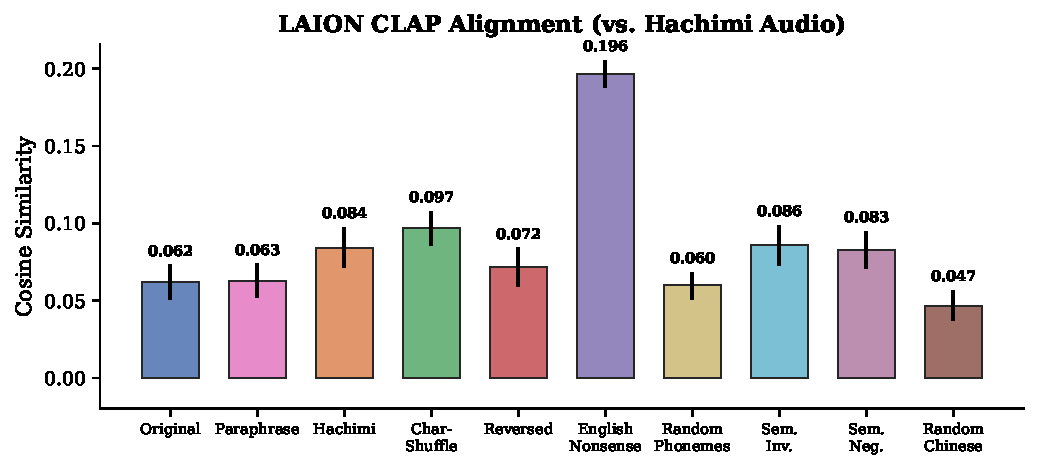
\includegraphics[width=\linewidth]{figures/fig1_alignment.pdf}
\caption{LAION CLAP alignment across all conditions (vs.\ hachimi audio). Error bars: 95\% bootstrap CIs. Original lyrics and paraphrases are indistinguishable ($d{=}{-}0.02$), both significantly below hachimi nonsense ($d{=}{-}0.24$--$0.25$). English nonsense achieves the highest alignment due to training data bias.}
\label{fig:alignment}
\end{figure}

\subsection{Cross-Model Comparison}\label{sec:crossmodel}

The semantic insensitivity observed above may reflect LAION CLAP's English-centric training rather than a general property of audio-text models. We test this with Microsoft CLAP~\citep{elizalde2024msclap}, which uses a different architecture (1024-dim vs.\ 512-dim) and was trained on broader multilingual data. Our primary evidence comes from LAION CLAP (full text, no truncation); msCLAP serves as a supplementary comparison with an important caveat.

\begin{table}[!t]
\centering
\caption{Cross-model comparison. All three models agree that hachimi text produces higher alignment than originals or paraphrases. Both LAION CLAP variants cannot distinguish originals from paraphrases (standard: $d{=}{-}0.02$; fused: $d{=}0.14$, both n.s.). msCLAP shows C0${>}$C8 ($d{=}0.45$), but this is confounded by text-length truncation (see text).}
\label{tab:crossmodel}
\scriptsize
\begin{adjustbox}{max width=\columnwidth}
\begin{tabular}{l ccc}
\toprule
\textbf{Condition} & \textbf{LAION} & \textbf{LAION-Fused} & \textbf{MS-CLAP} \\
\midrule
Original Lyrics & 0.062 [0.051, 0.073] & 0.031 [0.029, 0.032] & 0.228 [0.216, 0.241] \\
Paraphrase      & 0.063 [0.052, 0.074] & 0.030 [0.028, 0.032] & 0.197 [0.186, 0.209] \\
Hachimi            & 0.084 [0.071, 0.097] & 0.031 [0.029, 0.033] & 0.253 [0.238, 0.267] \\
Char-Shuffle       & 0.097 [0.086, 0.108] & --- & 0.242 [0.232, 0.253] \\
Reversed           & 0.072 [0.059, 0.084] & --- & 0.217 [0.204, 0.230] \\
Eng.\ Nonsense    & 0.196 [0.188, 0.205] & --- & 0.255 [0.243, 0.268] \\
Random Phonemes    & 0.060 [0.051, 0.068] & --- & 0.186 [0.178, 0.194] \\
Sem.\ Inversion    & 0.086 [0.073, 0.099] & --- & 0.252 [0.237, 0.266] \\
Sem.\ Negation     & 0.083 [0.070, 0.095] & --- & 0.234 [0.221, 0.247] \\
Random Chinese     & 0.047 [0.037, 0.056] & --- & 0.192 [0.182, 0.202] \\
\midrule
Original vs Hachimi: $d$ & $-0.24$ & $-0.37$ & $-0.27$ \\
Original vs Paraphrase: $d$ & $-0.02$ & $0.14$ & $0.45$ \\
\bottomrule
\end{tabular}
\end{adjustbox}
\end{table}

Table~\ref{tab:crossmodel} reveals that all three models agree on the key comparison: hachimi nonsense text produces higher alignment than both original lyrics and paraphrases (LAION: $d{=}{-}0.24$; LAION-Fused: $d{=}{-}0.37$; msCLAP: $d{=}{-}0.27$). Both LAION CLAP variants, which process full text without truncation, cannot distinguish originals from paraphrases (standard: $d{=}{-}0.02$, $p{=}0.82$; fused: $d{=}0.14$, $p{=}0.08$). We note that the fused result does not establish a general architectural theorem about cross-modal fusion; it shows only that enabling fusion layers in this specific LAION checkpoint did not restore paraphrase sensitivity. msCLAP shows a moderate original--paraphrase separation ($d{=}0.45$, $p{<}0.001$), but this result is confounded: text truncation to 500 characters affects 62\% of originals (mean 925 chars) but only 3\% of paraphrases (mean 277 chars), so the separation may reflect length differences rather than semantic sensitivity. The C0${<}$C1 ordering is consistent across all three models regardless of truncation.

The C0${\approx}$C8${<}$C1 pattern in both LAION CLAP variants provides the primary evidence: meaning-preserving rewording has no effect on alignment, while replacing meaning with rhythmic nonsense \emph{increases} it. The hachimi advantage likely reflects phonological properties (repeated short syllables with high rhythmic regularity) that create stronger cross-modal correlations with the audio signal than variable-length, semantically rich lyrics.

The English nonsense dominance is LAION-specific (msCLAP: C4 only marginally higher than C1, $d{=}0.06$), suggesting that LAION CLAP's high alignment for English text reflects tokenizer-level rather than semantic effects.

\begin{figure}[!t]
\centering
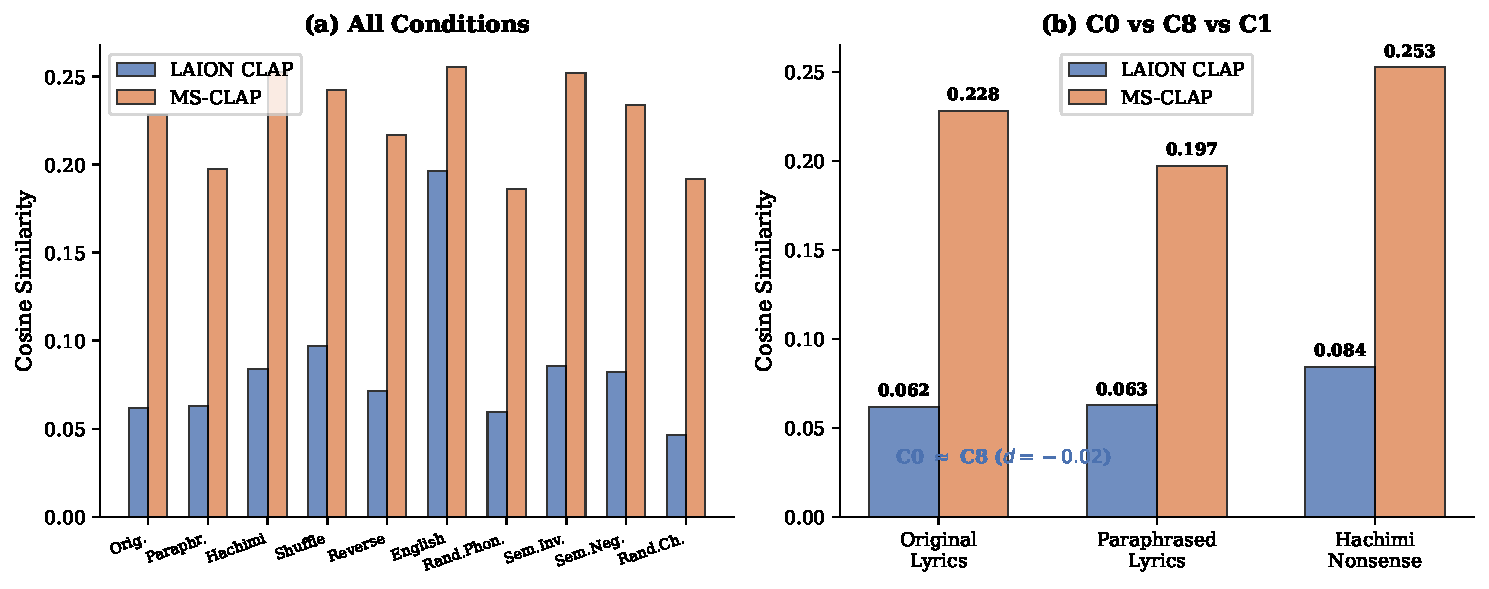
\includegraphics[width=\linewidth]{figures/fig7_cross_model.pdf}
\caption{Cross-model comparison. All three models show hachimi nonsense (C1) achieving higher alignment than originals (C0) and paraphrases (C8). Both LAION CLAP variants cannot distinguish originals from paraphrases. Error bars: 95\% bootstrap CIs.}
\label{fig:crossmodel}
\end{figure}

\subsection{Temporal Matching Control}\label{sec:temporal}

The full-song analysis above uses complete audio files, where hachimi and original versions may differ in duration and temporal structure. To test whether the C0${<}$C1 pattern is an artifact of temporal misalignment, we extract temporally matched segments using chroma cross-correlation: for each hachimi-original pair, we identify the time window in the original that best matches the hachimi recording (quality filters: $z$-score${\geq}2.0$, feature similarity${\geq}0.55$, cross-validation agreement). This yields 107 matched pairs (64\% of 166 songs; kept and dropped songs show indistinguishable C0--C1 gaps, $t{=}{-}0.36$, $p{=}0.72$, ruling out selection bias).

On temporally matched segments, the C0${<}$C1 pattern in LAION CLAP persists: original lyrics achieve alignment of 0.028, hachimi 0.052 ($d{=}0.27$, $p{=}0.006$, 95\% CI [0.015, 0.066]). The per-song C0--C1 gap correlates strongly with the full-song gap ($r{=}0.80$, $p{<}0.001$), with 81\% of songs agreeing in gap direction. The gap is slightly larger for segments than full songs (0.024 vs.\ 0.020) but this difference is not significant ($p{=}0.49$). Segment duration does not predict the gap ($r{=}0.07$, $p{=}0.48$), and match quality metrics ($z$-score, feature similarity) are not significant predictors in a multiple regression ($R^{2}{=}0.66$, only full-song gap significant, $p{<}0.001$). These results indicate that the C0${<}$C1 pattern is not explained by coarse temporal misalignment.

For msCLAP, the matched-segment analysis reveals a model-specific boundary condition: the C0${<}$C1 effect holds with hachimi audio ($d{=}{-}0.24$, $p{=}0.014$) but not with temporally matched original audio ($d{=}{-}0.02$, $p{=}0.85$). In LAION CLAP, the effect is consistent across both audio sources ($d{=}0.27$ vs.\ $d{=}0.23$, both $p{<}0.05$, not significantly different, $p{=}0.45$). This suggests that msCLAP's alignment is more sensitive to audio-specific acoustics, while LAION CLAP's C0${<}$C1 effect is robust to the audio source.

\subsection{Acoustic Properties and Sensitivity Analysis}\label{sec:acoustic}

Having established that LAION CLAP alignment is insensitive to meaning-preserving paraphrases, we investigate what does influence it.

\paragraph{What predicts alignment?}
We extract 57-dimensional acoustic feature vectors from each audio file (\S\ref{sec:audio_features}) and compute per-song Pearson correlations with CLAP alignment scores. Three MFCC coefficients survive Bonferroni correction: MFCC-7 ($r{=}{-}0.36$, $p_{\text{bonf}}{<}0.001$), MFCC-9 ($r{=}{-}0.31$, $p_{\text{bonf}}{=}0.002$), and MFCC-0 ($r{=}{-}0.26$, $p_{\text{bonf}}{=}0.04$). Hachimi and original recordings share near-identical acoustic profiles (cosine${=}0.999$), explaining why text variation has no effect: both texts are paired with acoustically identical audio.

\paragraph{Embedding geometry.}
A potential confound is that cosine similarity may be dominated by modality-specific directions in the embedding space. To test this, we apply ZCA whitening separately to text and audio embeddings. This removes all alignment (max${=}0.008$), confirming that CLAP's alignment is carried by the learned cross-modal correlation structure in the joint space rather than by isotropic, modality-independent features. Critically, this result does not isolate semantic contributions: whitening removes the entire covariance structure, making it impossible to attribute the alignment loss to any specific factor (semantic or otherwise). Rather, it serves as a geometry check, confirming that the alignment signal resides in the learned principal directions of the joint space.

\paragraph{Vocal-only audio.}
With full-mix audio, instruments may dominate the signal and mask text contribution. Using separated vocal tracks, LAION CLAP produces significant original--hachimi separation ($d{=}{-}0.47$, $p{<}.001$), consistent with msCLAP ($d{=}{-}1.32$). This resolves the apparent contradiction: the full-mix effect ($d{=}{-}0.24$) is attenuated by instrumental dominance, but the direction is consistent (Appendix~\ref{fig:vocal}).

\paragraph{Spectral perturbation analysis.}
To test whether acoustic spectral features influence alignment, we perturb original audio in three ways ($N{=}80$ songs, Table~\ref{tab:perturbation}). Pitch shift and time stretch produce non-significant changes for Chinese text ($\Delta{<}0.02$) but significant changes for English nonsense ($\Delta{\approx}0.06$, $d{\approx}0.71$), suggesting CLAP's English-text pathway is more acoustically sensitive. Lowpass filtering \emph{increases} alignment for Chinese text ($\Delta{=}{-}0.051$, $d{=}{-}0.54$) but not for English nonsense ($\Delta{=}0.019$, n.s.). This is consistent with high-frequency spectral content introducing text-audio mismatch for Chinese text; lowpass filtering removes this mismatching component. Modality dominance analysis shows roughly equal contribution ($|\Delta_{\text{audio}}|/|\Delta_{\text{text}}|{=}1.06$, $p{=}0.49$).

\begin{table}[!t]
\centering
\caption{Audio perturbation sensitivity analysis ($N{=}80$). $\Delta$ = reference $-$ perturbed. Lowpass filtering increases alignment for Chinese text, consistent with spectral content influencing CLAP alignment.}
\label{tab:perturbation}
\scriptsize
\begin{adjustbox}{max width=\columnwidth}
\begin{tabular}{l r r r l}
\toprule
\textbf{Perturbation} & \textbf{Text} & $\boldsymbol{\Delta}$ & $\boldsymbol{d}$ & \textbf{Sig.} \\
\midrule
\multirow{3}{*}{Pitch shift (+3 st.)}
  & Orig.\ lyrics & $+0.016$ & $0.16$ & n.s. \\
  & Hachimi & $+0.016$ & $0.17$ & n.s. \\
  & English nons.\ & $+0.061$ & $0.71$ & $p{<}0.001$ \\
\midrule
\multirow{3}{*}{Time stretch ($\times$1.2)}
  & Orig.\ lyrics & $+0.001$ & $0.01$ & n.s. \\
  & Hachimi & $+0.019$ & $0.20$ & n.s. \\
  & English nons.\ & $+0.065$ & $0.71$ & $p{<}0.001$ \\
\midrule
\multirow{3}{*}{Lowpass filter (3\,kHz)}
  & Orig.\ lyrics & $-0.051$ & $-0.54$ & $p{<}0.001$ \\
  & Hachimi & $-0.034$ & $-0.35$ & $p{<}0.01$ \\
  & English nons.\ & $+0.019$ & $0.21$ & n.s. \\
\bottomrule
\end{tabular}
\end{adjustbox}
\end{table}

\subsection{Phonology Control via Homophone Replacement}\label{sec:homophone}

To partially isolate phonological from semantic contributions, we introduce a \emph{homophone} condition: each Chinese character in the original lyrics is replaced with a \emph{different} character that has the \emph{same} pinyin (pronunciation). This preserves phonological structure (same syllables, same tones) while destroying semantic meaning. If CLAP alignment is driven purely by phonology, homophones should match originals; if character identity or semantics matter, homophones should differ.

The homophone replacement achieves an average substitution rate of 65.3\% of characters. LAION CLAP alignment for the homophone condition (mean${=}0.051$, 95\% CI [0.040, 0.063]) is significantly \emph{lower} than original lyrics ($d{=}{-}0.27$, $p{<}0.001$, Wilcoxon $p{=}0.002$), with homophones winning only 39.2\% of per-song comparisons. Critically, homophones also have lower alignment than paraphrases (C8: $d{=}{-}0.17$, $p{=}0.028$).

This result is informative: preserving phonology alone is \emph{not} sufficient to maintain alignment—changing characters while keeping the same sounds decreases alignment. This suggests that CLAP's text encoder processes features beyond pure phonology, including orthographic or lexical surface-form properties. Combined with the C0$\approx$C8 result (changing words while keeping meaning has \emph{no} effect), the pattern suggests that LAION CLAP's alignment is sensitive to text surface form in ways that are not reducible to either semantics or phonology alone.

\subsection{msCLAP Truncation Control}\label{sec:truncation}

Microsoft CLAP shows a C0--C8 separation ($d{=}0.45$, $p{<}0.001$) that could reflect semantic sensitivity or text-length differences (C0 mean${\approx}925$ chars vs.\ C8 mean${\approx}277$ chars with 500-char truncation). To disentangle these factors, we rerun msCLAP with length-matched text: both C0 and C8 are truncated to \emph{min(C0\_len, C8\_len, 500)} per song, equalizing maximum text length.

With length-matched truncation, the C0--C8 gap persists: $d{=}0.38$ ($p{<}0.001$), only slightly reduced from the standard truncation ($d{=}0.44$). The hachimi advantage (C1${>}$C0) also survives ($d{=}{-}0.32$, $p{<}0.001$). This confirms that msCLAP's original--paraphrase separation is not a truncation artifact: even with identical text length, msCLAP distinguishes paraphrases from originals. This contrasts with LAION CLAP's C0$\approx$C8 result, suggesting that msCLAP's multilingual training encodes surface-form features that LAION CLAP does not capture. Both models agree on the hachimi advantage (C1${>}$C0).

% ============================================================
\section{Discussion}\label{sec:discussion}
% ============================================================

\paragraph{Observational findings, not causal claims.}
We emphasize that this study is \emph{observational}: hachimi lyrics naturally bundle semantic removal with phonological, rhythmic, and tokenization changes, making it impossible to isolate semantics as a single causal factor. The C0/C8 comparison provides the cleanest available test of semantic sensitivity, but even paraphrases may differ in singability, lexical rarity, and stylistic naturalness. Our results are therefore best interpreted as a case study of how CLAP behaves under a specific class of natural lyric perturbations, rather than a definitive decomposition of semantic versus acoustic contributions. Whether the observed insensitivity reflects CLAP's limited text encoder capacity or a fundamental property of contrastive alignment objectives remains an open question. The probing classifier result (CLAP 71.2\% vs.\ BERT 90.3\% accuracy) is suggestive but not conclusive evidence for the capacity-limitation hypothesis.

\paragraph{Why does this matter?}
Despite these caveats, the observational findings have practical implications for music information retrieval systems that use CLAP for zero-shot classification or text-to-music retrieval. The paraphrase result suggests that LLM-generated text descriptions may align poorly with audio even when semantically correct, because they lack the phonological and rhythmic properties of natural song text. The retrieval analysis (C0 Recall@1 $<$ 2\%) demonstrates that meaningful lyrics rarely rank highest among conditions, which raises concerns about whether CLAP captures semantic content in music settings. These observations motivate further controlled experiments with cleaner variable isolation.

\paragraph{Limitations.}
Several caveats apply. First, our sample of 166 songs limits statistical power for detecting small effects; bootstrap CIs for some conditions span roughly 30\% of the mean (e.g., LAION C1: [0.071, 0.097]). Future work should scale to 1{,}000+ pairs. Second, the hachimi vs.\ original comparison confounds semantics with phonology and prosody; isolating semantics would require TTS-generated audio with identical prosody. Third, the whitening result (alignment depends on cross-modal correlation structure) means the ``semantic insensitivity'' may reflect embedding geometry rather than absent capability; models with better-balanced joint spaces might differ. Fourth, our dataset is drawn from Chinese internet-culture music and we test only two CLAP variants. Fifth, the paraphrase control is generated by an LLM (Qwen2.5-7B) and may not preserve all aspects of meaning; the observed alignment difference between originals and paraphrases could partly reflect generation artifacts. Future work includes TTS-based phonology controls, testing additional architectures, and extending to larger multilingual datasets.

% ============================================================
\section{Conclusion}\label{sec:conclusion}
% ============================================================

Using hachimi lyrics and a ten-condition degeneration spectrum across three CLAP variants and 166 paired songs, we show that CLAP variants exhibit \emph{model-dependent} sensitivity to lyric surface form in Chinese music: preserving meaning or phonology alone is insufficient to predict alignment behavior. Both LAION CLAP variants cannot distinguish meaning-preserving paraphrases from originals (standard: $d{=}{-}0.02$; fused: $d{=}0.14$, both n.s.), while Microsoft CLAP does ($d{=}0.45$, confounded by text length), showing that paraphrase sensitivity is model-dependent rather than universal. Nonsense hachimi lyrics produce moderately higher alignment across all three models ($d{=}{-}0.24$ to $-0.37$), though this comparison also confounds semantics with phonological changes. These findings are specific to the tested models and Chinese-language lyric data; generalization to other models, languages, or audio domains requires further investigation. They highlight the importance of controlling for phonological regularity and acoustic confounds in multimodal alignment evaluation.

% ============================================================
\bibliography{references}

\appendix

\section{Degeneration Spectrum Conditions}\label{app:conditions}

\begin{table}[!h]
\centering
\caption{Ten conditions of the degeneration spectrum. C8 (paraphrase) is the semantic control.}
\label{tab:conditions}
\small
\begin{adjustbox}{max width=\columnwidth}
\begin{tabular}{lll}
\toprule
\textbf{Condition} & \textbf{Operation} & \textbf{Tests} \\
\midrule
Original Lyrics    & Original meaningful lyrics         & Semantic baseline \\
Paraphrase         & LLM rewording, same meaning        & \textbf{Semantic control} \\
Hachimi             & Nonsense hachimi lyrics             & Non-semantic baseline \\
Char-Shuffle        & Characters scrambled within words   & Orthographic cues \\
Reversed            & Word segments reversed              & Sequential structure \\
English Nonsense    & English syllable walk                & Cross-lingual phonotactics \\
Random Phonemes     & Random Chinese syllables             & Phonetic texture \\
Sem.\ Inversion     & Negations in hachimi               & Sem.\ ops on non-semantic \\
Sem.\ Negation      & Negations in original lyrics         & Sem.\ ops on meaningful \\
Random Chinese      & Random common characters            & Structure-free control \\
\bottomrule
\end{tabular}
\end{adjustbox}
\end{table}

\section{Paraphrase Quality Validation}\label{app:paraphrase}

\begin{table}[!h]
\centering
\caption{Quality metrics for LLM-generated paraphrases ($N{=}165$). High semantic similarity confirms meaning preservation; low character Jaccard confirms different surface forms.}
\label{tab:paraphrase_quality}
\small
\begin{tabular}{l r}
\toprule
\textbf{Metric} & \textbf{Value} \\
\midrule
Semantic similarity (orig vs paraphrase) & $0.84 \pm 0.11$ \\
Character Jaccard overlap & $0.37$ \\
Paraphrase length (mean chars) & $292$ \\
Original length (mean chars, cleaned) & $929$ \\
\bottomrule
\end{tabular}
\end{table}

\section{Acoustic Feature Correlations}\label{app:acoustic}

\begin{table}[!h]
\centering
\caption{Top acoustic features correlated with hachimi alignment. Three MFCC coefficients survive Bonferroni correction ($\alpha{=}0.05/57{=}0.0009$).}
\label{tab:acoustic_full}
\small
\begin{adjustbox}{max width=\columnwidth}
\begin{tabular}{l r r r}
\toprule
\textbf{Feature} & $r$ & $p$ & $p_{\text{bonf}}$ \\
\midrule
MFCC-7 (timbre)          & $-0.36$ & $2 \times 10^{-6}$ & $1 \times 10^{-4}$ \\
MFCC-9 (timbre)          & $-0.31$ & $4 \times 10^{-5}$ & $2 \times 10^{-3}$ \\
MFCC-0 (energy envelope) & $-0.26$ & $6 \times 10^{-4}$ & $4 \times 10^{-2}$ \\
MFCC-5 (timbre)          & $-0.24$ & $2 \times 10^{-3}$ & $9 \times 10^{-2}$ \\
Dynamic range            & $-0.22$ & $5 \times 10^{-3}$ & $3 \times 10^{-1}$ \\
\bottomrule
\end{tabular}
\end{adjustbox}
\end{table}

\section{Whitening Analysis}\label{app:whitening}

\begin{table}[!h]
\centering
\caption{Alignment before and after ZCA whitening (vs.\ hachimi audio). All differences $p{<}10^{-13}$.}
\label{tab:whitening}
\small
\begin{adjustbox}{max width=\columnwidth}
\begin{tabular}{l r r r}
\toprule
\textbf{Condition} & \textbf{Original} & \textbf{Whitened} & $\boldsymbol{d}$ \\
\midrule
Original Lyrics   & 0.060 & 0.003 & $0.82$ \\
Hachimi            & 0.084 & $-$0.005 & $0.96$ \\
Char-Shuffle       & 0.097 & 0.001 & $1.18$ \\
Reversed           & 0.072 & 0.004 & $0.79$ \\
English Nonsense   & 0.196 & $-$0.002 & $2.57$ \\
Random Phonemes    & 0.060 & $-$0.001 & $0.75$ \\
Sem.\ Inversion    & 0.086 & $-$0.001 & $0.97$ \\
Sem.\ Negation     & 0.083 & 0.008 & $0.84$ \\
Random Chinese     & 0.047 & $-$0.005 & $0.63$ \\
\bottomrule
\end{tabular}
\end{adjustbox}
\end{table}

\section{Permutation Test}\label{app:permutation}

\begin{table}[!h]
\centering
\caption{Permutation test (10{,}000 shuffles). The C0--C1 difference is significant under permutation, confirming that the relative ordering is robust. Both conditions show weak absolute alignment.}
\label{tab:permutation}
\small
\begin{adjustbox}{max width=\columnwidth}
\begin{tabular}{l r r}
\toprule
\textbf{Comparison} & $\boldsymbol{d}$ & $\boldsymbol{p}$ \\
\midrule
Original vs.\ Hachimi & $-0.24$ & $0.001$ \\
Original vs.\ Paraphrase & $-0.02$ & $0.82$ \\
\bottomrule
\end{tabular}
\end{adjustbox}
\end{table}

\section{Hyperparameters and Reproducibility}\label{app:hyperparams}

\begin{table}[!h]
\centering
\caption{Model configurations and hyperparameters.}
\label{tab:hyperparams}
\small
\begin{tabular}{l l}
\toprule
\textbf{Parameter} & \textbf{Value} \\
\midrule
\multicolumn{2}{l}{\textbf{LAION CLAP}} \\
Architecture & HTSAT-base \\
Embedding dim & 512 \\
Training data & LAION-Audio-630K \\
\multicolumn{2}{l}{\textbf{LAION CLAP (Fused)}} \\
Architecture & HTSAT-base + fusion layers \\
Embedding dim & 512 \\
Fusion & Cross-modal fusion enabled \\
\multicolumn{2}{l}{\textbf{Microsoft CLAP}} \\
Architecture & HTSAT-full \\
Embedding dim & 1024 \\
Training data & MusicCaps + various \\
\multicolumn{2}{l}{\textbf{BERT-base-Chinese}} \\
Layers & 12, hidden 768 \\
Pooling & Mean-pooled last hidden state \\
\multicolumn{2}{l}{\textbf{HuBERT-base}} \\
Layers & 12, hidden 768 \\
Pooling & Last hidden state \\
CCA components & 50 \\
\multicolumn{2}{l}{\textbf{Validation}} \\
Semantic similarity model & text2vec-base-chinese \\
\multicolumn{2}{l}{\textbf{Experimental}} \\
Random seed & 42 \\
Audio sample rate & 22,050\,Hz \\
Audio duration & 60s \\
Bootstrap iterations & 10,000 \\
Permutation shuffles & 10,000 \\
Bonferroni $\alpha$ & 0.05 \\
Paraphrase model & Qwen2.5-7B (local) \\
Paraphrase truncation & 500 characters \\
msCLAP text truncation & 500 characters \\
\bottomrule
\end{tabular}
\end{table}

\paragraph{Code and Data.}
Code and data processing scripts are available at \url{https://github.com/[anon]/hachimi-alignment}. Audio files are subject to copyright; we provide song metadata and all text conditions.

\begin{figure}[!h]
\centering
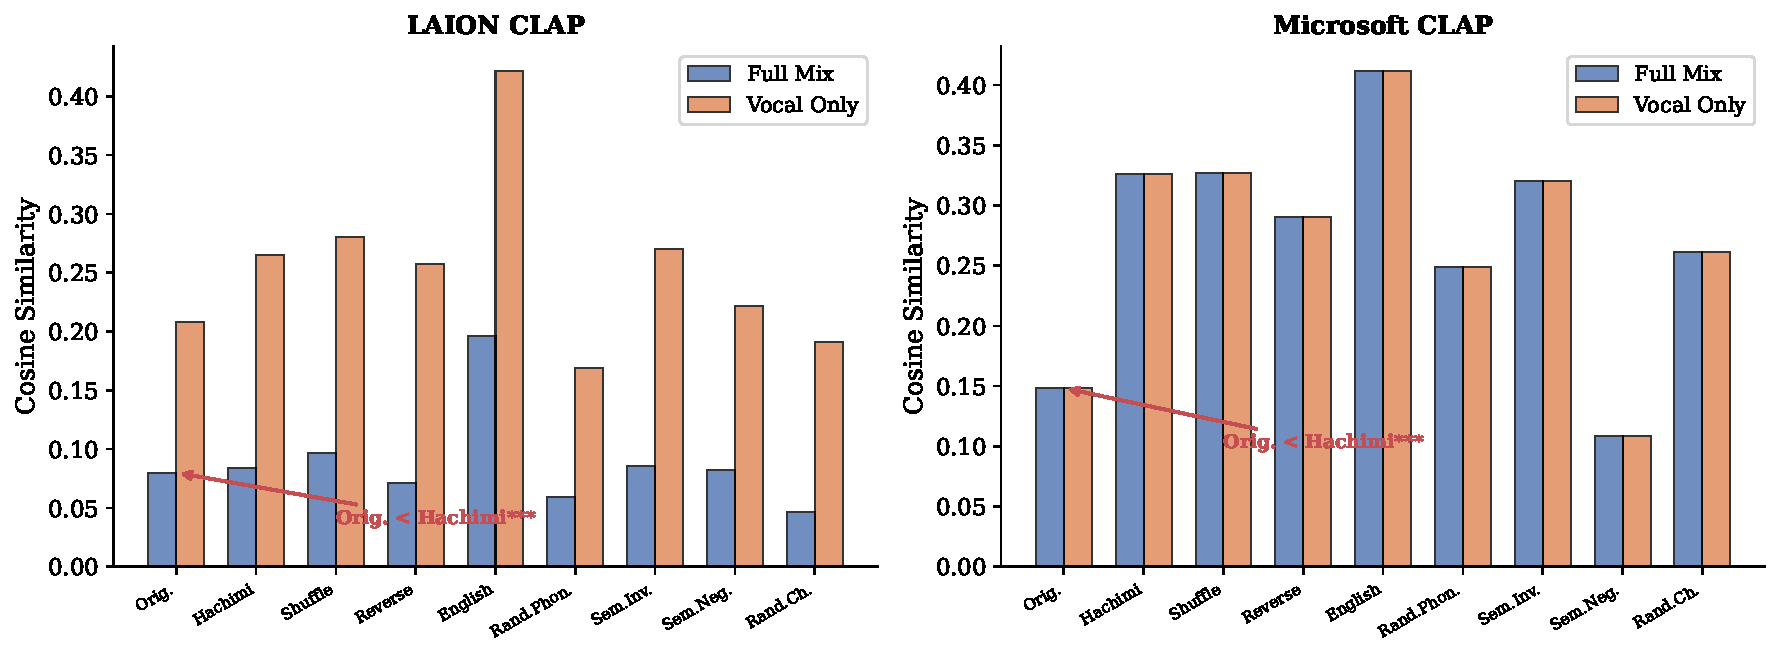
\includegraphics[width=\linewidth]{figures/fig8_vocal_only.pdf}
\caption{Full-mix vs.\ vocal-only alignment. Removing instruments amplifies the original${<}$hachimi separation in LAION CLAP (left), matching msCLAP's direction (right).}
\label{fig:vocal}
\end{figure}

\end{document}
